\appendix

\section{Mathematical Review}

This appendix reviews some of the mathematical concepts used in this
manual.

\subsection{Rotation transforms}
\label{Rotations:sec}

Rotation matrices are used to describe the orientation of 3D
coordinate frames in space, and to transform vectors between these
coordinate frames.

\begin{figure}[t]
\begin{center}
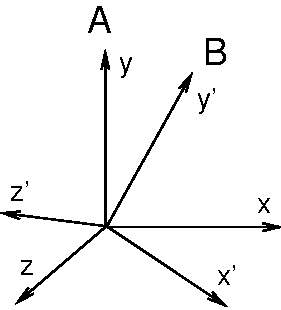
\includegraphics[width=2in]{images/rotationAB}
\end{center}
\caption{Two coordinate frames A and B rotated with respect
to each other.}
\label{rotationAB:fig}
\end{figure}

Consider two 3D coordinate frames A and B that are rotated with
respect to each other (Figure \ref{rotationAB:fig}).  The orientation
of B with respect to A can be described by a $3 \times 3$ rotation
matrix $\R_{BA}$, whose columns are the unit vectors giving the
directions of the rotated axes $\x'$, $\y'$, and $\z'$ of B with
respect to A.

$\R_{BA}$ is an {\it orthogonal} matrix, meaning that
its columns are both perpendicular and mutually
orthogonal, so that
%
\begin{equation}
\R_{BA}^T \, \R_{BA} = \I
\end{equation}
%
where $\I$ is the $3 \times 3$ identity matrix. The inverse
of $\R_{BA}$ is hence equal to its transpose:
%
\begin{equation}
\R_{BA}^{_1} = \R_{BA}^T
\label{RABinv:eqn}
\end{equation}
%
Because $\R_{BA}$ is orthogonal, $|\det \R_{BA}| = 1$, and because it
is a rotation, $\det \R_{BA} = 1$. The other case, where $\det \R_{BA}
= -1$, is not a rotation but a {\it reflection}.
The 6 orthogonality constraints associated with a rotation matrix mean
that in spite of having 9 numbers, the matrix only has 3 degrees of
freedom.

Now, assume we have a 3D vector $\v$, and consider its coordinates
with respect to both frames A and B.  Where necessary, we use a
preceding superscript to indicate the coordinate frame with repect to
which a quantity is described, so that ${}^A\v$ and ${}^B\v$ and
denote $\v$ with respect to frames A and B, respectively.  Given the
definition of $\R_{AB}$ given above, it is fairly straightforward to
show that
%
\begin{equation}
{}^A\v = \R_{BA} \, {}^B\v
\label{vectorTransform:eqn}
\end{equation}
%
and, given (\ref{RABinv:eqn}), that
%
\begin{equation}
{}^B\v = \R_{BA}^T \, {}^A\v.
\label{vectorInvTransform:eqn}
\end{equation}
%
Hence in addition to describing the orientation of B with respect to A,
$\R_{BA}$ is also a transformation matrix that maps vectors in B
to vectors in A.

It is straightforward to show that
%
\begin{equation}
\R_{BA}^{-1} = \R_{BA}^T = \R_{AB}.
\label{rotationInverse:eqn}
\end{equation}
%

\begin{figure}[t]
\begin{center}
 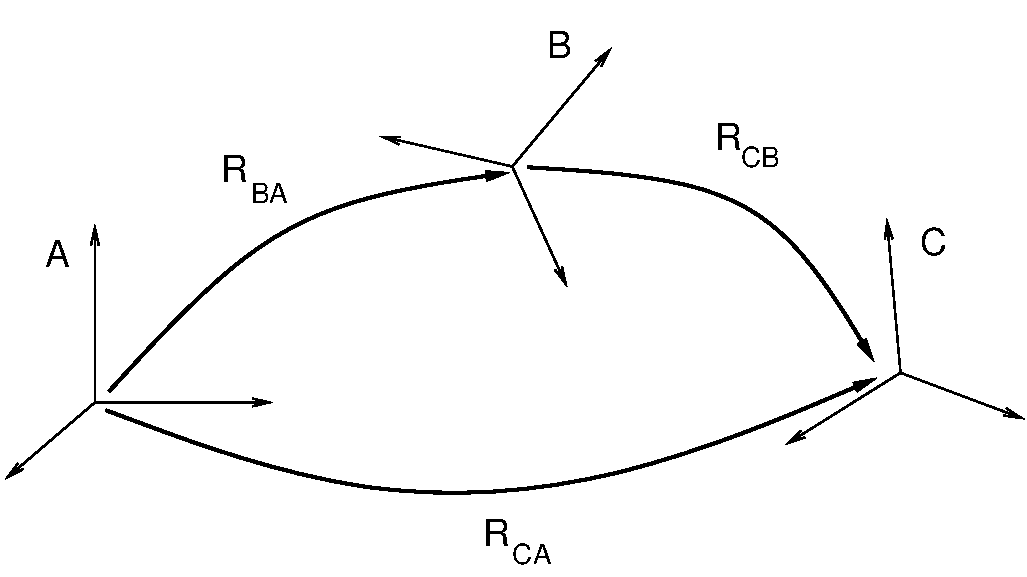
\includegraphics[width=4.5in]{images/rotationsABC}
\end{center}
\caption{Schematic illustration of three coordinate frames A, B, and C
and the rotational transforms relating them.}
\label{rotationsABC:fig}
\end{figure}

A simple rotation by an angle $\theta$ about one of the basic
coordinate axes known as a {\it basic} rotation. The three
basic rotations about x, y, and z are:
%
\begin{equation*}
\R_x(\theta) = \matl 1 & 0 & 0 \\ 
               0 & \cos(\theta) & -\sin(\theta) \\ 
               0 & \sin(\theta) & \cos(\theta) 
		 \matr
\end{equation*}
%
\begin{equation*}
\R_y(\theta) = \matl \cos(\theta) & 0 & \sin(\theta) \\ 
               0 & 1 & 0 \\ 
               -\sin(\theta) & 0 & \cos(\theta) 
                 \matr
\end{equation*}
%
\begin{equation*}
\R_z(\theta) = \matl \cos(\theta) & -\sin(\theta) & \\ 
               \sin(\theta) & \cos(theta) & 0 \\ 
               0 & 0 & 1 
                 \matr
\label{elementaryRotations:sec}
\end{equation*}
%

Next, we consider transform composition. Suppose we have three
coordinate frames, A, B, and C, whose orientation are related to each other by
$\R_{BA}$, $\R_{CB}$, and $\R_{CA}$ (Figure
\ref{transformsABC:fig}).  If we know $\R_{BA}$ and $\R_{CA}$,
then we can determine $\R_{CB}$ from
%
\begin{equation}
\R_{CB} = \R_{BA}^{-1} \, \R_{CA}.
\label{rotationCB:eqn}
\end{equation}
%
This can be understood in terms of vector transforms. $\R_{CB}$
transforms a vector from C to B, which is equivalent to first
transforming from C to A,
%
\begin{equation}
{}^A\v = \R_{CA} \, {}^C\v,
\end{equation}
%
and then transforming from A to B:
%
\begin{equation}
{}^B\v = \R_{BA}^{-1} \, {}^A\v = \R_{BA}^{-1} \; \R_{CA} {}^C\v = \R_{CB} \, {}^C\v.
\end{equation}
%
Note also from (\ref{rotationInverse:eqn}) that $\R_{CB}$ can be 
expressed as
%
\begin{equation}
\R_{CB} = \R_{AB} \, \R_{CA}.
\label{rotationCBII:eqn}
\end{equation}
%

In addition to specifying rotation matrix components explicity,
there are numerous other ways to describe a rotation.
Three of the most common are:

\begin{description}

\item[Roll-pitch-yaw angles]\mbox{}

There are 6 variations of roll-pitch-yaw angles. The one used in
ArtiSynth corresponds to older robotics texts (e.g., Paul, Spong) and
consists of a roll rotation $r$ about the z axis, followed by a pitch
rotation $p$ about the new y axis, followed by a yaw rotation $y$
about the new x axis. The net rotation can be expressed by the
following product of basic rotations: $\R_z(r) \, \R_y(p) \, \R_x(y)$.

\item[Axis-angle]\mbox{}

An axis angle rotation parameterizes a rotation as a rotation by
an angle $\theta$ about a specific axis $\u$. Any rotation
can be represented in such a way as a consequence of Euler's rotation
theorem.

\item[Euler angles]\mbox{}

There are 6 variations of Euler angles. The one used in ArtiSynth
consists of a rotation $\phi$ about the z axis, followed by a rotation
$\theta$ about the new y axis, followed by a rotation $\psi$ about the
new z axis. The net rotation can be expressed by the following product
of basic rotations: $\R_z(\phi) \, \R_y(\theta) \, \R_z(\psi)$.

\end{description}

\subsection{Rigid transforms}
\label{RigidTransforms:sec}

Rigid transforms are used to specify both the transformation of points
and vectors between coordinate frames, as well as the relative
position and orientation between coordinate frames.

\begin{figure}[h]
\begin{center}
 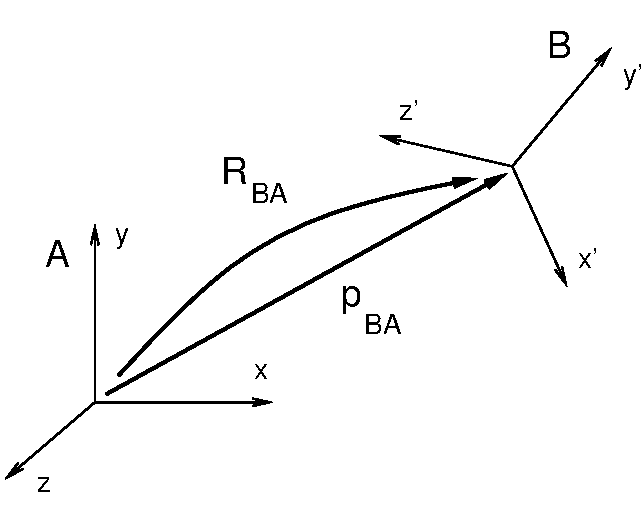
\includegraphics[width=3.25in]{images/framesAB}
\end{center}
\caption{A position vector $\p_{BA}$ and rotation matrix
$\R_{BA}$ describing the position and orientation of frame B
with respect to frame A.}
\label{framesAB:fig}
\end{figure}

Consider two 3D coordinate frames in space, A and B (Figure
\ref{framesAB:fig}). The translational position of B with respect to A
can be described by a vector $\p_{BA}$ from the origin of A to the
origin of B (described with respect to frame A). Meanwhile, the
orientation of B with respect to A can be described by the $3 \times
3$ rotation matrix $\R_{BA}$ (Section \ref{Rotations:sec}).  The
combined position and orientation of B with respect to A is known as
the {\it pose} of B with respect to A.

\begin{figure}[t]
\begin{center}
 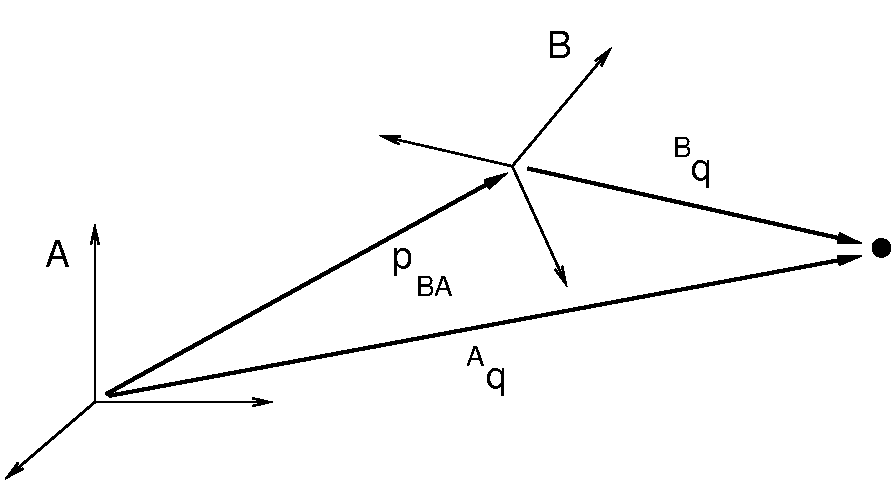
\includegraphics[width=3.75in]{images/pointsAB}
\end{center}
\caption{Point vectors ${}^A\q$ and ${}^B\q$ describing
the position of a point $\q$ with respect to frames A and B.}
\label{pointsAB:fig}
\end{figure}

Now, assume we have a 3D point $\q$, and consider its coordinates with
respect to both frames A and B (Figure \ref{pointsAB:fig}). Given the
pose descriptions given above, it is fairly straightforward to show
that
%
\begin{equation}
{}^A\q = \R_{BA} \, {}^B\q + \p_{BA}
\label{pointTransform:eqn}
\end{equation}
%
and, given (\ref{RABinv:eqn}), that
%
\begin{equation}
{}^B\q = \R_{BA}^T \, ({}^A\q - \p_{BA}).
\label{pointInvTransform:eqn}
\end{equation}
%

If we extend our points into a 4D {\it homogeneous} coordinate space
with the fourth coordinate $w$ equal to 1, i.e.,
%
\begin{equation}
\q^* \equiv \matl \q \\ 1 \matr,
\end{equation}
%
then (\ref{pointTransform:eqn}) and
(\ref{pointInvTransform:eqn}) can be simplified to
%
\begin{equation*}
{}^A\q^* = \T_{BA} \, {}^B\q^* \quad \text{and} \quad
{}^B\q^* = \T_{BA}^{-1} \, {}^A\q^*
\end{equation*}
%
where
%
\begin{equation}
\T_{BA} = \matl \R_{BA} & \p_{BA} \\ 0 & 1 \matr
\end{equation}
%
and
%
\begin{equation}
\T_{BA}^{-1} = \matl \R_{BA}^T & -\R_{BA}^T \p_{BA} \\ 0 & 1 \matr.
\end{equation}
%
$\T_{BA}$ is the $4 \times 4$ {\it rigid transform matrix} that
transforms points from B to A and also describes the pose of
B with respect to A (Figure \ref{transformAB:fig}).

\begin{figure}[t]
\begin{center}
 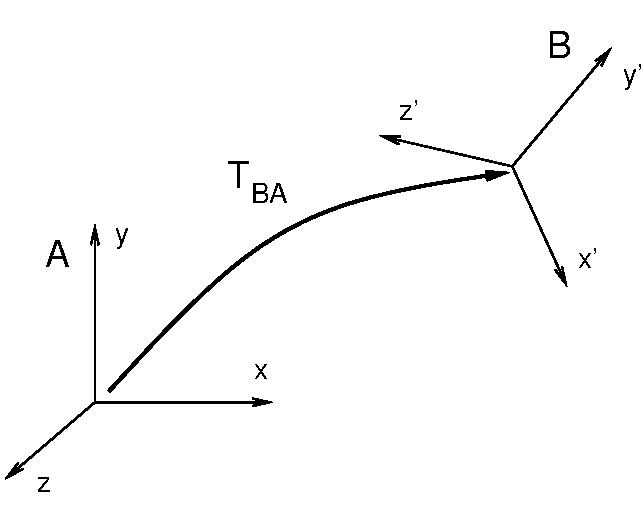
\includegraphics[width=3in]{images/transformAB}
\end{center}
\caption{The transform matrix $\T_{BA}$ from B to A.}
\label{transformAB:fig}
\end{figure}

It is straightforward to show that $\R_{BA}^T$ and $-\R_{BA}^T
\p_{BA}$ describe the orientation and position of $A$ with respect to
$B$, and so therefore
%
\begin{equation}
\T_{BA}^{-1} = \T_{AB}.
\label{transformInverse:eqn}
\end{equation}
%

Note that if we are transforming a vector $\v$ instead of a point
between B and A, then we are only concerned about relative orientation
and the vector transforms (\ref{vectorTransform:eqn}) and
(\ref{vectorInvTransform:eqn}) should be used instead.
However, we can express these using $\T_{BA}$ if
we embed vectors in a homogeneous coordinate space 
with the fourth coordinate $w$ equal to 0, i.e.,
%
\begin{equation}
\v^* \equiv \matl \v \\ 0 \matr,
\end{equation}
%
so that
%
\begin{equation*}
{}^B\v^* = \T_{BA} \, {}^A\v^* \quad \text{and} \quad
{}^A\v^* = \T_{BA}^T \, {}^B\v^*.
\end{equation*}
%

\begin{figure}[t]
\begin{center}
 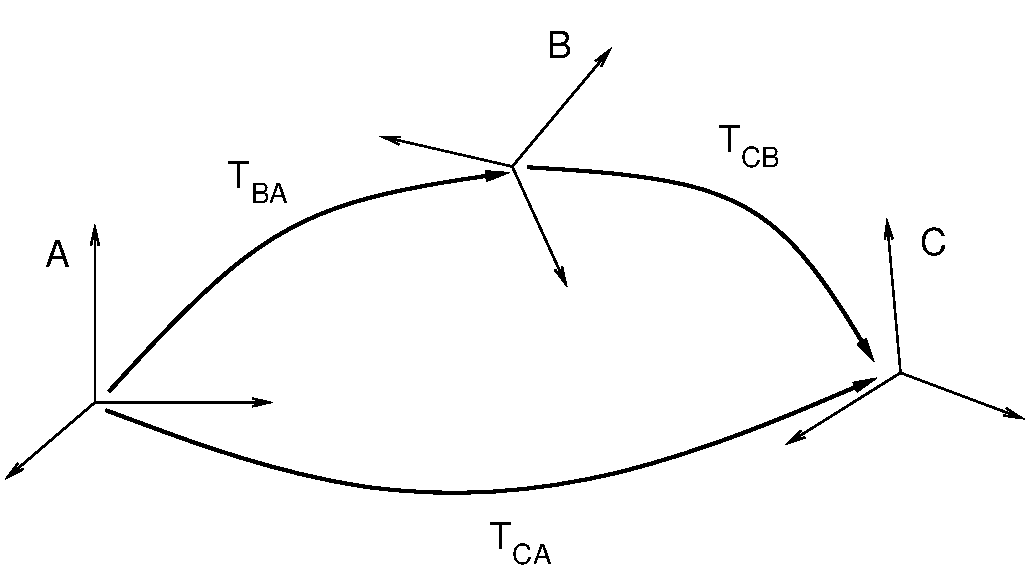
\includegraphics[width=4.5in]{images/transformABC}
\end{center}
\caption{Three coordinate frames A, B, and C and the transforms
relating each one to the other.}
\label{transformsABC:fig}
\end{figure}

Finally, we consider transform composition. Suppose we have three
coordinate frames, A, B, and C, each related to the other by
transforms $\T_{BA}$, $\T_{CB}$, and $\T_{CA}$ (Figure
\ref{transformsABC:fig}).  Using the same reasoning used to derive
(\ref{rotationCB:eqn}) and (\ref{rotationCBII:eqn}), it is easy to
show that
%
\begin{equation}
\T_{CB} = \T_{BA}^{-1} \; \T_{CA} = \T_{AB} \; \T_{CA}.
\end{equation}
%

\subsection{Affine transforms}
\label{AffineTransforms:sec}

An {\it affine transform} is a generalization of a rigid transform, in
which the rotational component $\R$ is replaced by a general $3 \times
3$ matrix $\A$. This means that an affine transform implements a
generalized basis transformation combined with an offset of the origin
(Figure \ref{affineAB:fig}). As with $\R$ for rigid transforms, the
columns of $\A$ still describe the transformed basis vectors $\x'$,
$\y'$, and $\z'$, but these are no longer guaranteed to orthonormal.

\begin{figure}[h]
\begin{center}
 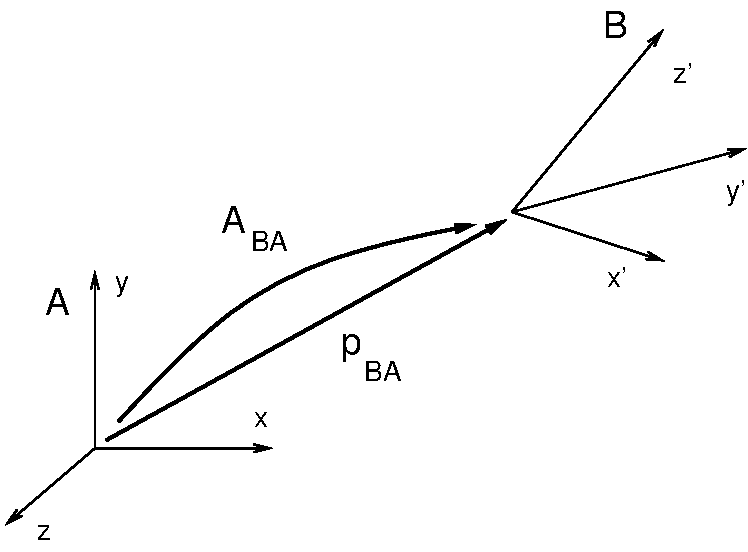
\includegraphics[width=3.25in]{images/affineAB}
\end{center}
\caption{A position vector $\p_{BA}$ and a general matrix $\A_{BA}$
describing the position and basis transform of frame B with respect to
frame A.}
\label{affineAB:fig}
\end{figure}

Expressed in terms of homogeneous coordinates,
the affine transform $\X_{AB}$ takes the form
%
\begin{equation}
\X_{BA} = \matl \A_{BA} & \p_{BA} \\ 0 & 1 \matr
\end{equation}
%
with
%
\begin{equation}
\X_{BA}^{-1} = \matl \A_{BA}^{-1} & -\A_{BA}^{\-1} \p_{BA} \\ 0 & 1 \matr.
\end{equation}
%
As with rigid transforms, when an affine transform is applied to a
vector instead of a point, only the matrix $\A$ is applied and the
translation component $\p$ is ignored.

Affine transforms are typically used to effect transformations that
require stretching and shearing of a coordinate frame.  By the polar
decomposition theorem, $\A$ can be factored into a regular
rotation $\R$ plus a symmetric shearing/scaling matrix $\P$:
%
\begin{equation}
\A = \R \, \P
\end{equation}
%
Affine transforms can also be used to perform reflections, in which
$\A$ is orthogonal (so that $\A^T \, \A = \I$) but with $\det \A =
-1$.

\subsection{Rotational velocity}

\begin{figure}[h]
\begin{center}
 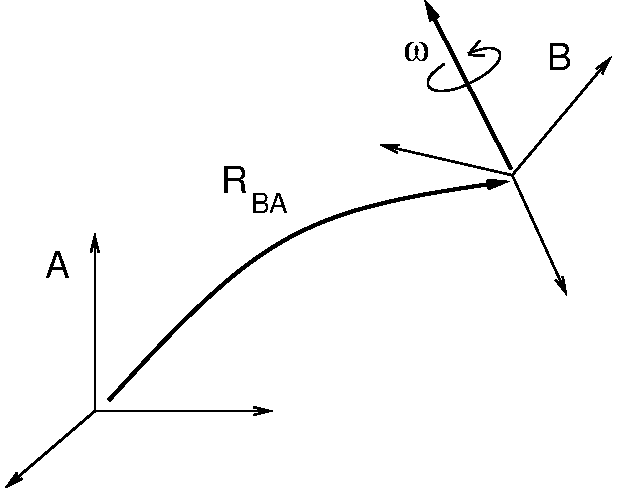
\includegraphics[width=3.25in]{images/angularvelAB}
\end{center}
\caption{Frame B rotating with respect to frame A.}
\label{angularvelAB:fig}
\end{figure}

Given two 3D coordinate frames A and B, the rotational, or {\it
angular}, velocity of B with respect to A is given by a 3D vector
$\Bom_{BA}$ (Figure \ref{angularvelAB:fig}). $\Bom_{BA}$
is related to the derivative of $\R_{BA}$ by
%
\begin{equation}
\dot\R_{BA} = [{}^A\Bom_{BA}] \R_{BA} = \R_{BA} [{}^B\Bom_{BA}]
\end{equation}
%
where ${}^A\Bom_{BA}$ and ${}^B\Bom_{BA}$ indicate $\Bom_{BA}$ with
respect to frames $A$ and $B$ and $[ \Bom ]$ denotes the $3 \times 3$
cross product matrix
%
\begin{equation}
[ \Bom ] \equiv 
\matl
0 & -\omega_z & \omega_y \\
\omega_z & 0 & -\omega_x \\
-\omega_y & \omega_x & 0 \\
\matr.
\label{xprodmatrix:eqn}
\end{equation}
%

If we consider instead the velocity of $A$ with respect to $B$, it is
straightforward to show that
%
\begin{equation}
\Bom_{AB} = -\Bom_{BA}. 
\end{equation}
%

\subsection{Spatial velocities and forces}
\label{SpatialVelocitiesAndForces:sec}

Given two 3D coordinate frames A and B, the {\it spatial velocity},
or {\it twist},
$\hat\v_{BA}$ of B with respect to A is given by the 6D 
composition of the translational velocity $\v_{BA}$ of the
origin of B with respect to A and the angular velocity $\Bom_{BA}$:
%
\begin{equation}
\hat\v_{BA} \equiv \matl \v_{BA} \\ \Bom_{BA} \matr.
\end{equation}
%
Similarly, the {\it spatial force}, or {\it wrench}, $\hat\f$ acting
on a frame B is given by the 6D composition of the translational force
$\f_B$ acting on the frame's origin and the moment $\Btau$, or torque,
acting through the frame's origin:
%
\begin{equation}
\hat\f_B \equiv \matl \f_B \\ \Btau_B \matr.
\end{equation}
%

\begin{figure}[h]
\begin{center}
 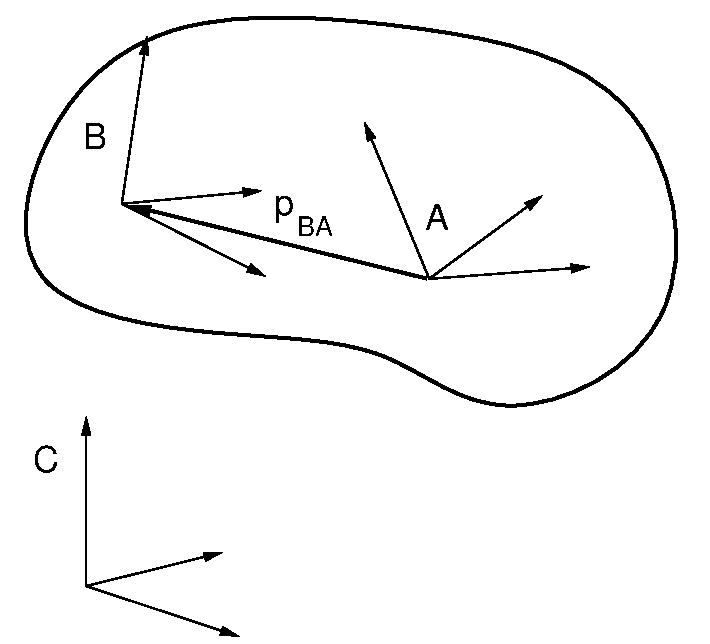
\includegraphics[width=3.25in]{images/rigidAB}
\end{center}
\caption{Two frames A and B rigidly connected within a rigid body
and moving with respect to a third frame C.}
\label{rigidAB:fig}
\end{figure}

If we have two frames $A$ and $B$ rigidly connected within a rigid
body (Figure \ref{rigidAB:fig}), and we know the spatial velocity
$\hat\v_{BC}$ of $B$ with respect to some third frame $C$, we may wish
to know the spatial velocity $\hat\v_{AC}$ of $A$ with respect to some
third frame $C$.  The angular velocity components are the same, but
the translational velocity components are coupled by the angular
velocity and the offset $\p_{BA}$ between $A$ and $B$, so that
%
\begin{equation*}
\v_{AC} = \v_{BC} - \p_{BA} \times \Bom_{BC}.
\end{equation*}
%
$\hat\v_{AC}$ is hence related to $\hat\v_{BC}$ via
\begin{equation*}
\matl \v_{AC} \\ \Bom_{AC} \matr =
\matl \I & -[\p_{BA}] \\ 0 & \I \matr \,
\matl \v_{BC} \\ \Bom_{BC} \matr.
\end{equation*}
%
where $[\p_{BA}]$ is defined by
(\ref{xprodmatrix:eqn}).

The above equation assumes that all quantities are expressed
with respect to the same coordinate frame.
If we instead consider $\hat\v_{AC}$ and $\hat\v_{BC}$ to be represented
in frames $A$ and $B$, respectively, then
we can show that
%
\begin{equation}
{}^A\hat\v_{AC} = \X_{BA} \, {}^B\hat\v_{BC},
\end{equation}
%
where
%
\begin{equation}
\X_{BA} \equiv
\matl \R_{BA} & -[\p_{BA}] \R_{BA} \\ 0 & \R_{BA} \matr.
\label{XvelAB:eqn}
\end{equation}
%
The transform $\X_{BA}$ is easily formed from the components of the
rigid transform $\T_{BA}$ relating $B$ to $A$.

The spatial forces $\hat\f_A$ and $\hat\f_B$ acting on frames $A$ and
$B$ within a rigid body are related in a similar way, only with
spatial forces, it is the moment that is coupled through the moment
arm created by $\p_{BA}$, so that
%
\begin{equation*}
\Btau_{A} = \Btau_{B} + \p_{BA} \times \f_{B}.
\end{equation*}
%
If we again assume that $\hat\f_A$ and $\hat\f_B$
are expressed in frames $A$ and $B$, we can show that
%
\begin{equation}
{}^A\hat\f_A = \X^*_{BA} \, {}^B\hat\f_B,
\end{equation}
%
where
%
\begin{equation}
\X^*_{BA} \equiv
\matl \R_{BA} & 0 \\  [\p_{BA}] \R_{BA} & \R_{BA} \matr.
\label{XforceAB:eqn}
\end{equation}
%

\subsection{Spatial inertia}
\label{SpatialInertia:sec}

Assume we have a rigid body with mass $m$ and a coordinate frame
located at the body's center of mass.  If $\v$ and $\Bom$ give the
translational and rotational velocity of the coordinate frame, then
the body's linear and angular momentum $\p$ and $\L$ are given by
%
\begin{equation}
\p = m \v \quad \text{and} \quad \L = \J \Bom,
\label{momenta:eqn}
\end{equation}
%
where $\J$ is the $3 \times 3$ {\it rotational inertia} with respect
to the center of mass. These relationships can be combined into a
single equation
%
\begin{equation}
\hat\p = \M \hat\v,
\label{momentum:eqn}
\end{equation}
%
where $\hat\p$ and $\M$ are the {\it spatial momentum} and
{\it spatial inertia}:
%
\begin{equation}
\hat\p \equiv \matl \p \\ \L \matr, \qquad
\M \equiv \matl m \I & 0 \\ 0 & \J \matr.
\end{equation}
%
The spatial momentum satisfies Newton's second law, so that
%
\begin{equation}
\hat\f = \frac{d \hat\p}{dt} = \M \frac{d \hat\v}{dt} + \dot\M \hat\v,
\end{equation}
%
which can be used to find the acceleration of a body in response to a
spatial force.

When the body coordinate frame is {\it not} located at the center of
mass, then the spatial inertia assumes the more complicated form
%
\begin{equation}
\matl 
m \I & -m [\c] \\ m [\c] & \J - m[\c][\c]
\matr,
\end{equation}
%
where $\c$ is the center of mass and $[\c]$ is defined by
(\ref{xprodmatrix:eqn}).

